\chapter{EXE stage}
\label{chap:exe}

In this stage it is performed the actual instructions' execution and the load/store memory address calculation.
Its general block diagram is shown in figure \ref{fig:EXE_stage}.

\begin{figure}[!ht]
	\centering
	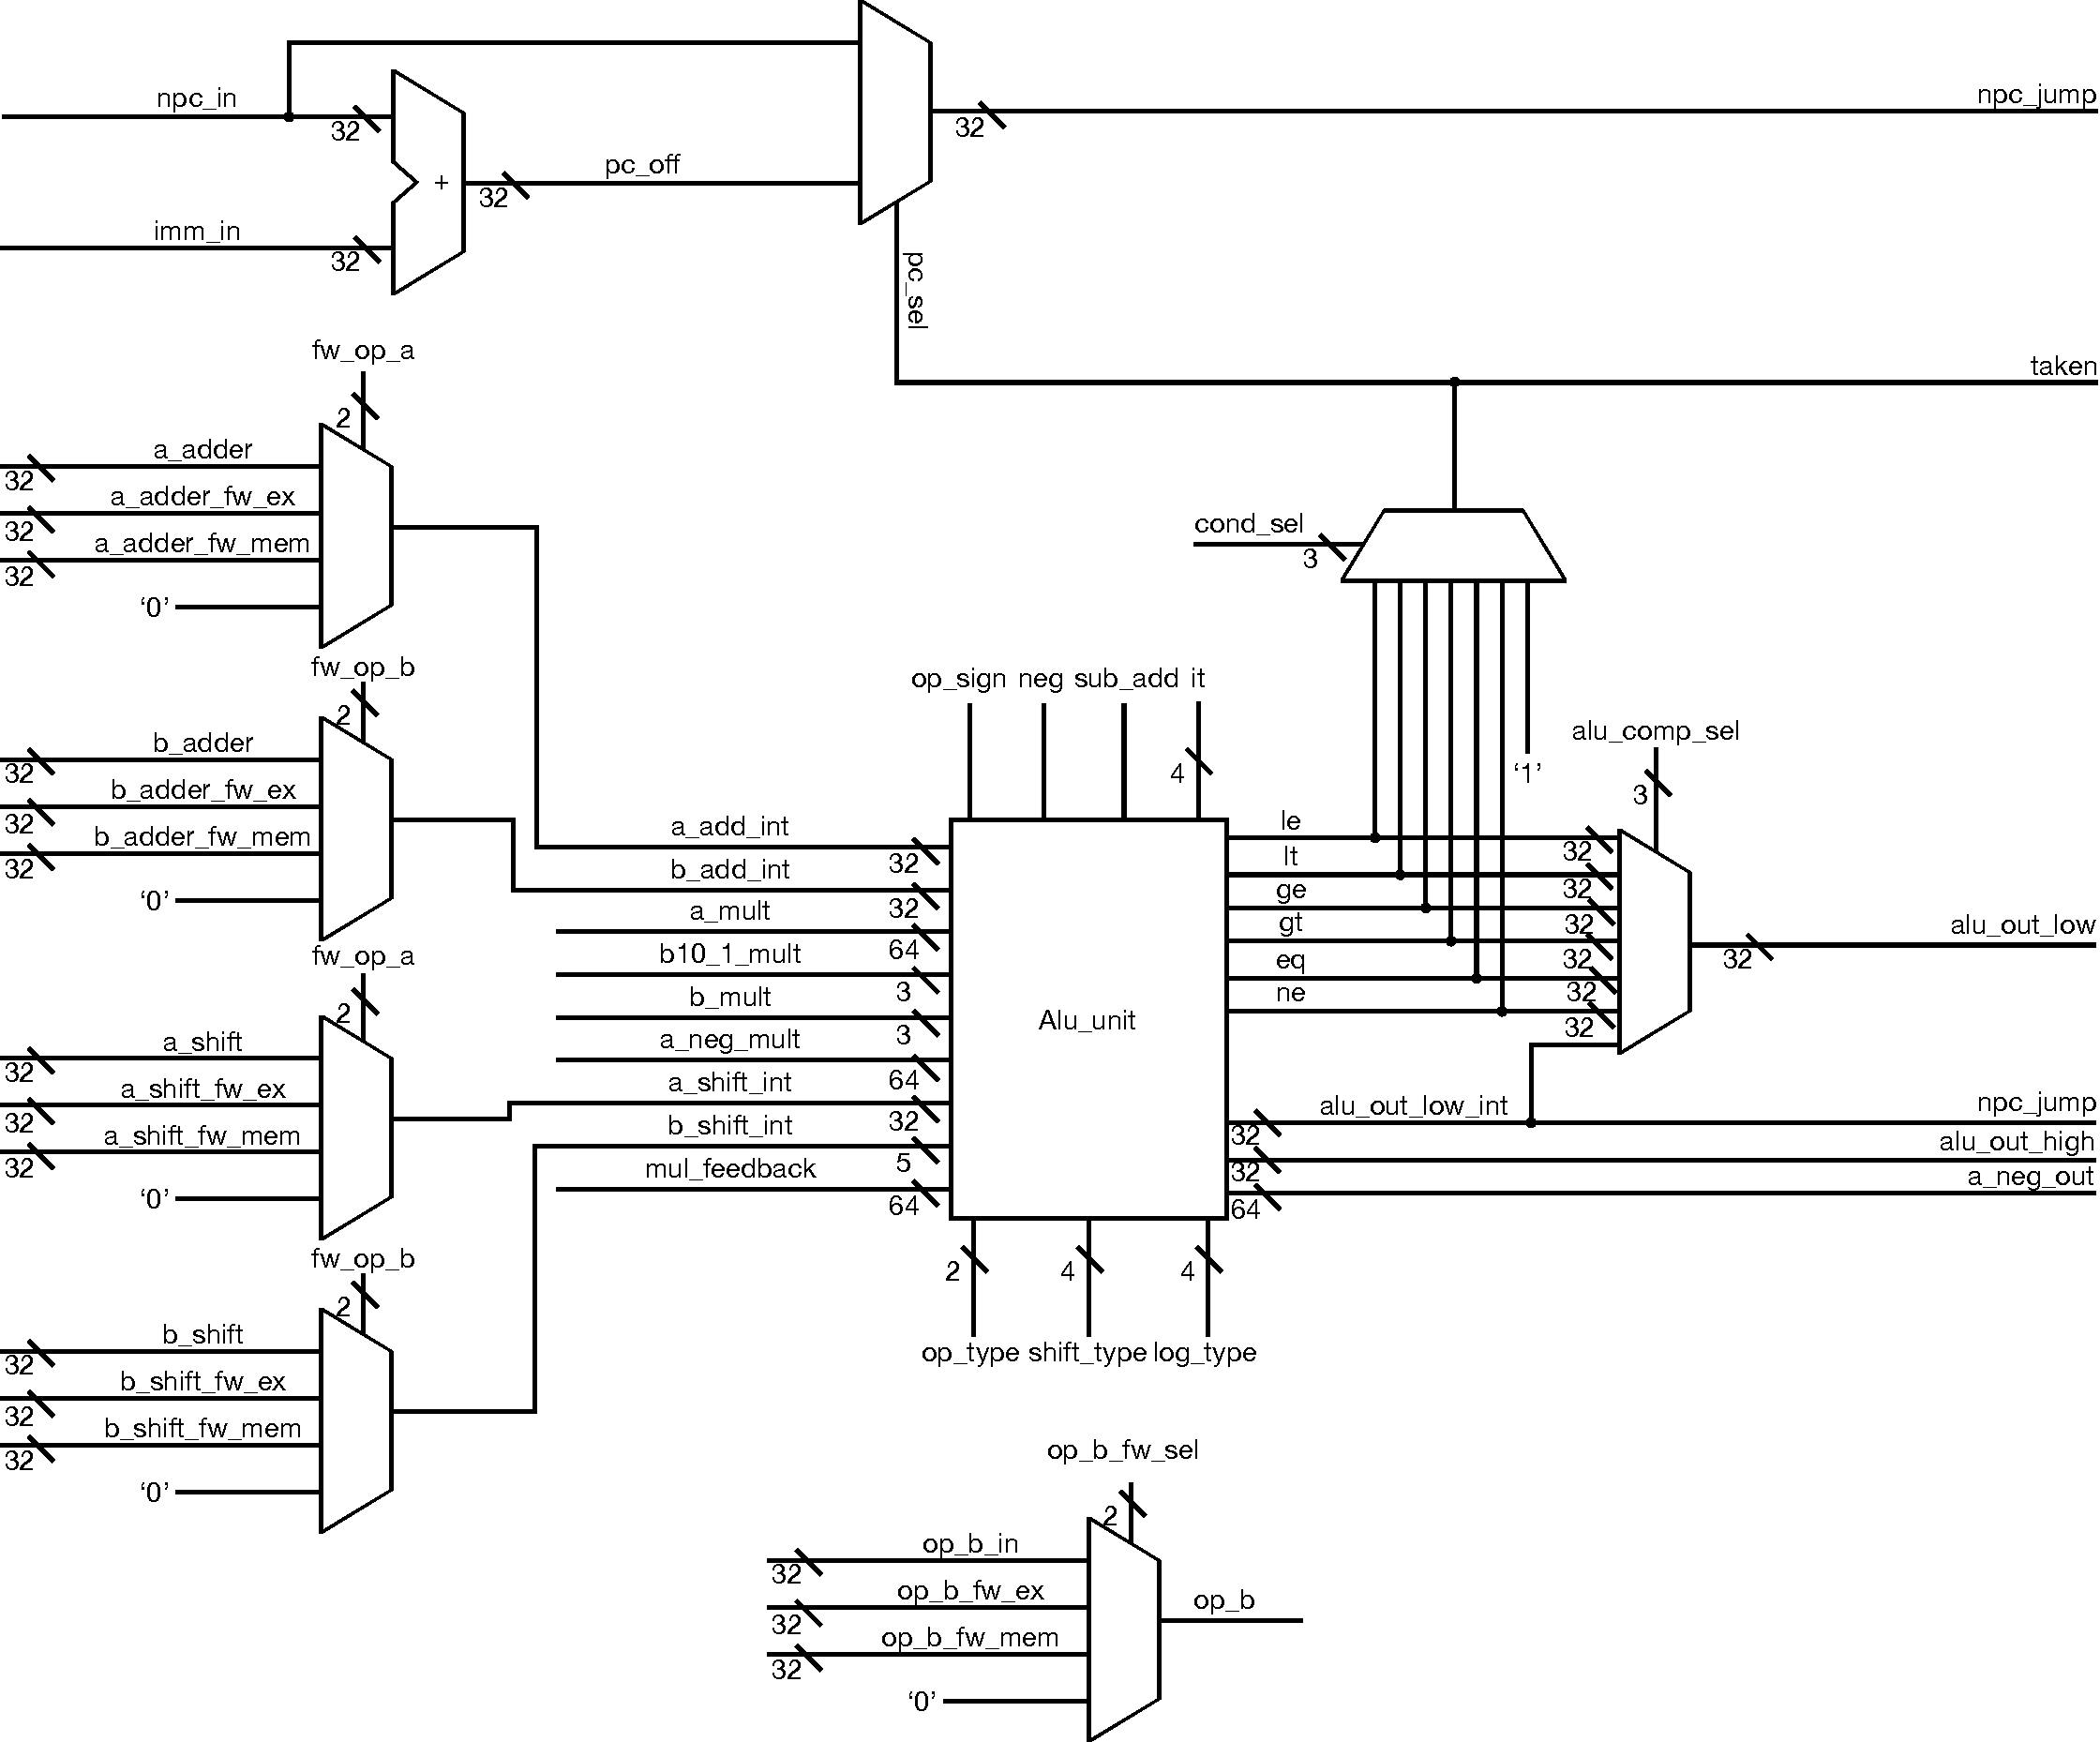
\includegraphics[width=0.8\linewidth]{./chapters/figures/ex_stage.pdf}
	\caption{Block diagram of the EXE stage}
	\label{fig:EXE_stage}
\end{figure}

The ALU incorporates the actual functional units, that are:

\begin{enumerate}
    \item an adder
    \item a shifter
    \item a logical unit
    \item a multiplier
\end{enumerate}

Each of these units have its own inputs coming from separate ID/EXE registers, the only exception being the adder and the logical units.
The rationale behind this is to reduce as much as possible the switching activity. These are, in fact, the most power hungry devices in the
whole datapath, therefore anything that can be done to reduce their power consumption leads to great benefits.

As it can be observed in the leftmost part of figure \ref{fig:EXE_stage}, the adder (and hence the logical), as well as the shifter, support forwarding.
Forwarding is also supported for the \verb|op_b| signal, that in case of a store contains the data to be written in cache.

At the center there is the ALU, discussed in details in section \ref{sec:alu}, and two muxes: the one that goes toward the top of the page is used to send
the \verb|taken| signal to the control unit in case of a branch execution and to drive the topmost mux, which outputs the correct value of the program counter.
The rightmost mux is, instead, used to select either the ALU's output signal or one of the internal comparator.

Finally, in the topmost part of figure \ref{fig:EXE_stage} there is a second adder, used to calculate $PC_{i+1} = PC_{i} + immediate$, where $i$ indicates the
current cycle number.

\section{ALU}
\label{sec:alu}

The ALU encapsulate, as said before, the various components that perform the wide range of supported operations. Its block diagram is shown in figure \ref{fig:alu}.

\begin{figure}[!ht]
	\centering
	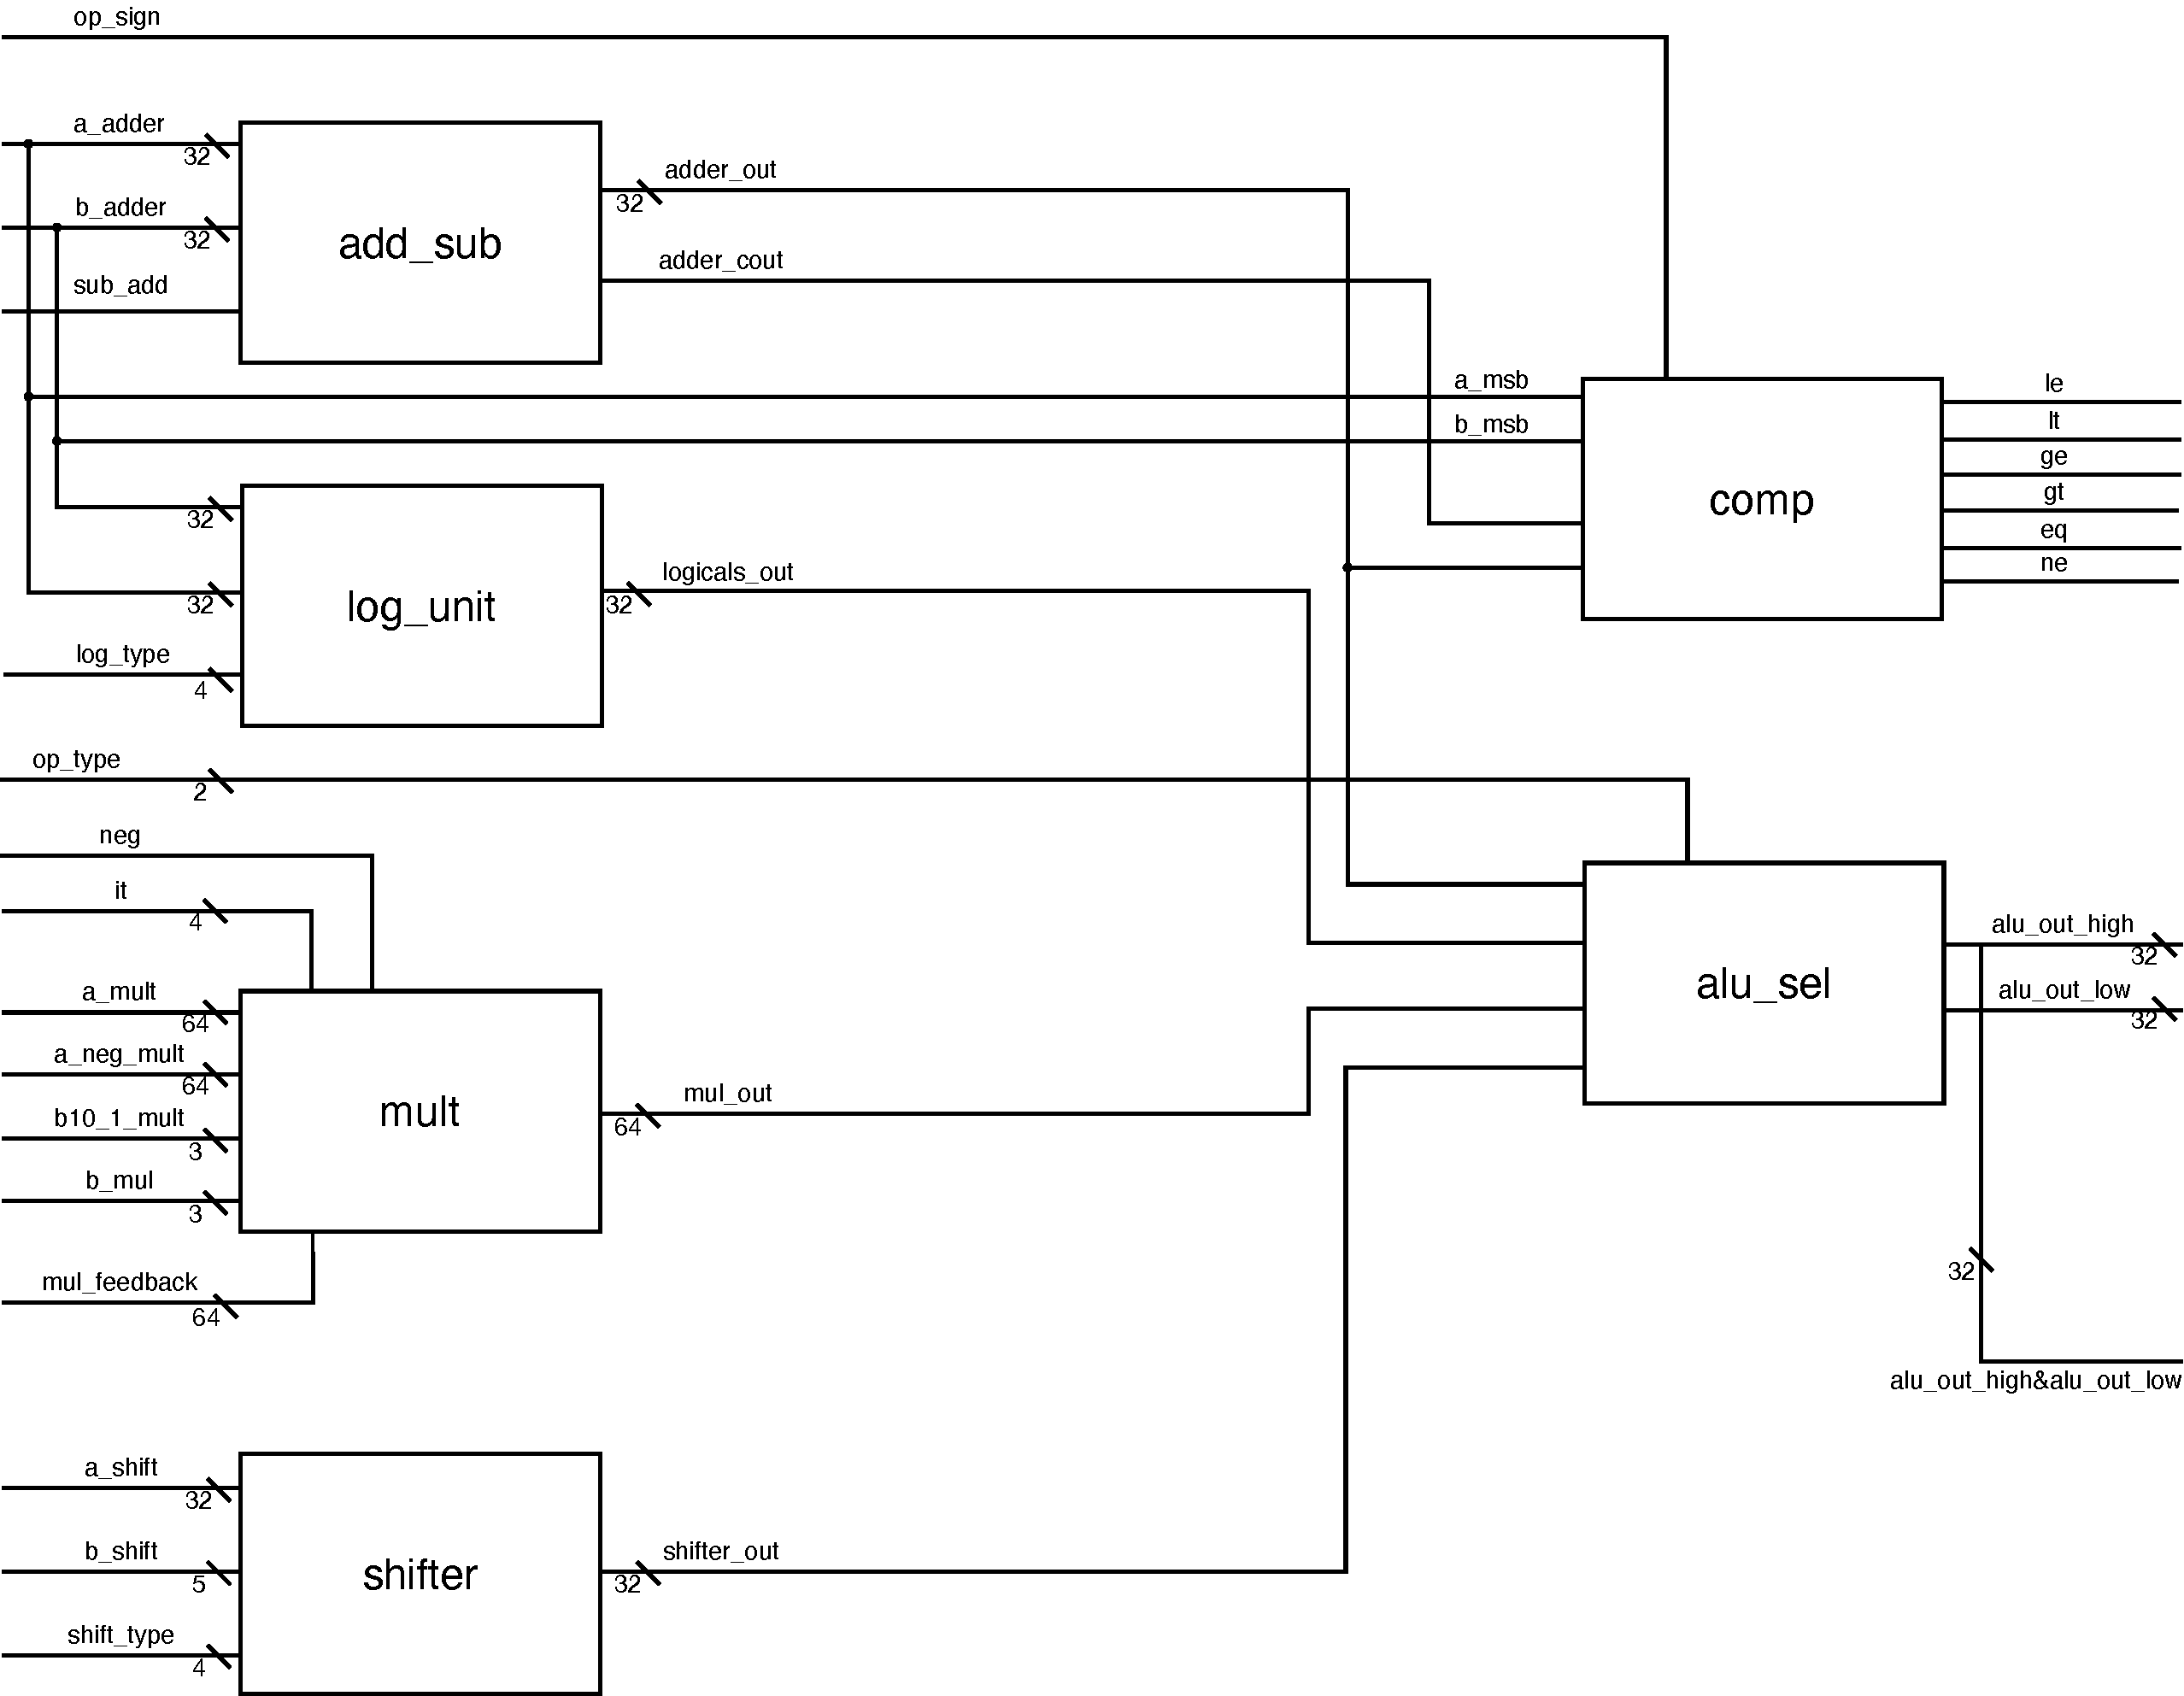
\includegraphics[width=0.8\linewidth]{./chapters/figures/ALU_exe.pdf}
	\caption{Block diagram of the ALU}
	\label{fig:alu}
\end{figure}

The adder, the logical unit and the shifter all implements structures seen during the lecture, in particular:

\begin{enumerate}
    \item the adder is an implementation of the P4.
    \item the logical unit implements the one seen inside the T2.
    \item the shifter is a smaller version than the one implemented in the T2.
\end{enumerate}

For this reasons, for the various images and explanation of these units refer to \cite{ln}.

\subsection{Multiplier}

The multiplication's algorithm is based on the Booth's algorithm explained during the lecture. However, we could not directly use the version developed for the laboratories.
Indeed, that was a fully combinational circuit, which delivered its result after $5\ ns$. It was too slow, big and power hungry. Hence, we modified the original structure in such
a way that it was pipelined and it used only a fraction of the components used in the original version. Its schematic is shown in figure \ref{fig:mul}

\begin{figure}[!ht]
	\centering
	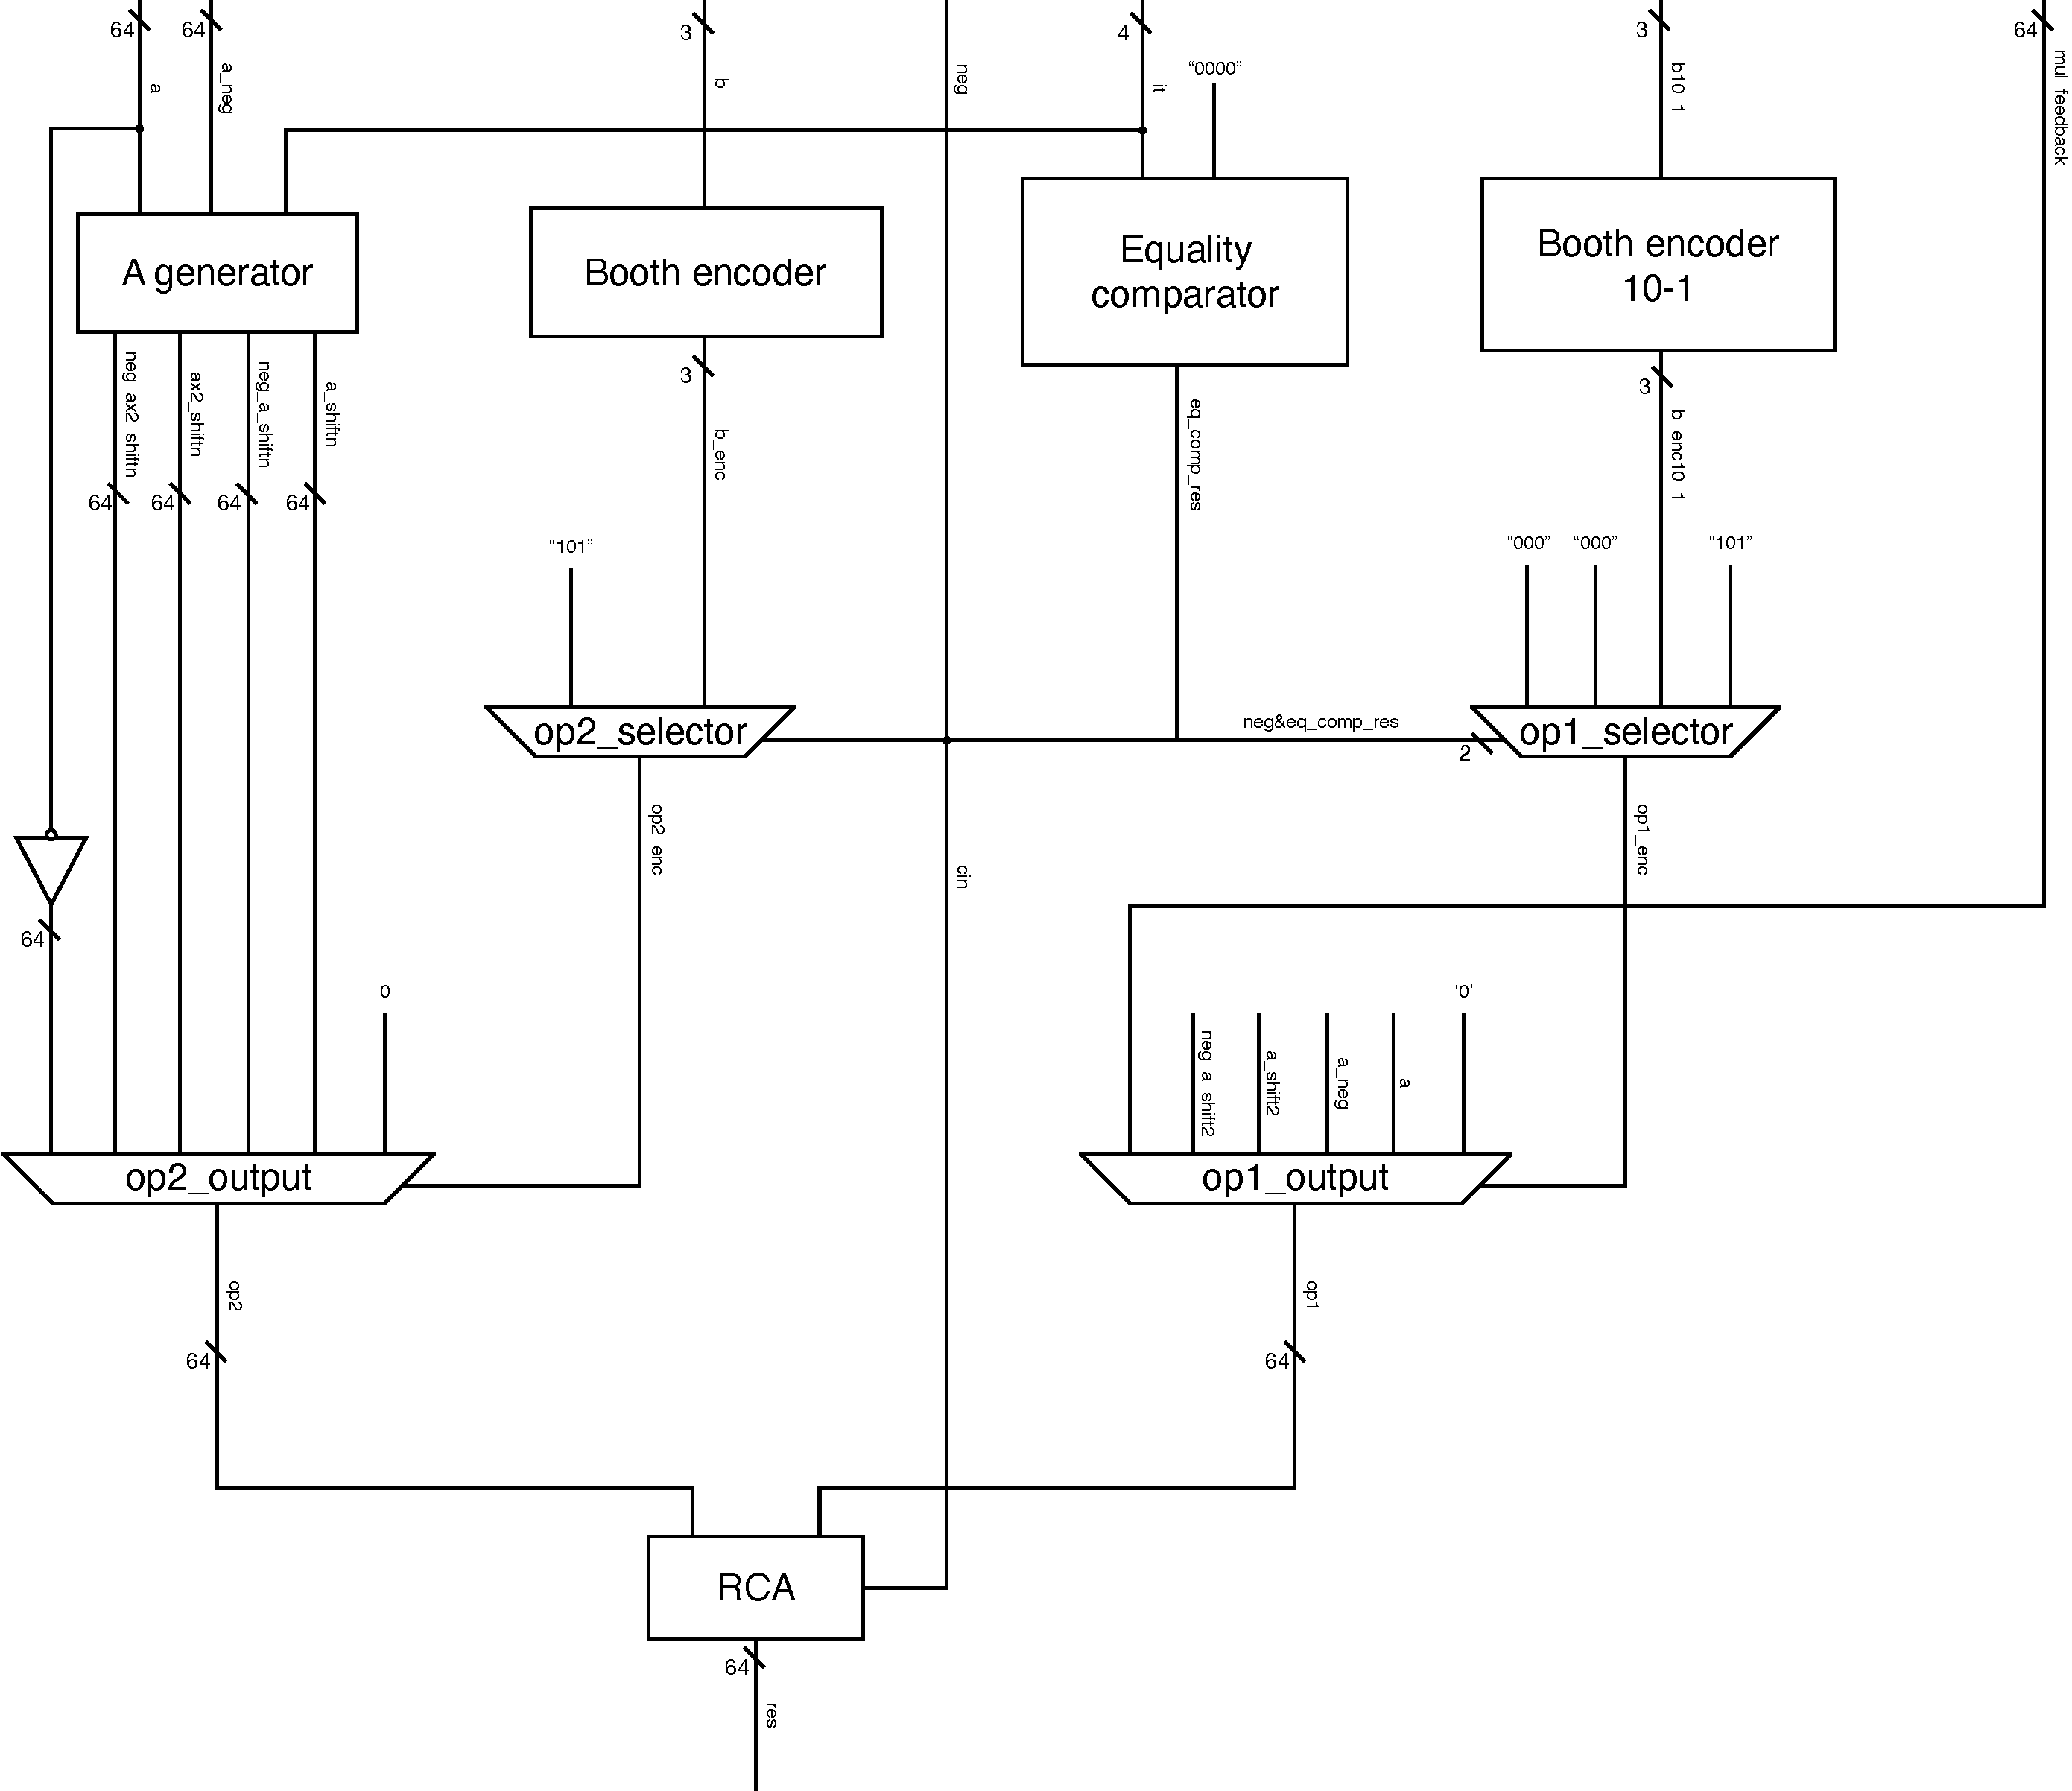
\includegraphics[width=0.8\linewidth]{./chapters/figures/mult.pdf}
	\caption{Multiplier schematic}
	\label{fig:mul}
\end{figure}

Overall it is composed by:

\begin{enumerate}
    \item a single 64-bits wide adder
    \item two 6 inputs muxes 64 bits wide
    \item one 4 inputs mux 3 bits wide
    \item one 2 inputs mux 3 bits wide
    \item an equality comparator
    \item two Booth's encoder
    \item a component called \verb|a_generator|
\end{enumerate}

It is clear that the area occupied is much smaller than the standard combinational version or even the pipelined one. This results also in huge power savings, since there are way
less components that contributes to $P_{leak}$.

Our algorithm works in this way:

\begin{enumerate}
    \item \textbf{Cycle 0}: The value of \verb|a| is extended on 64 bits and negated by the 64 bits adder. Then it is sampled by the corresponding ID/EXE register.
    \item \textbf{Cycle 1}: Both \verb|booth_encoder| and \verb|booth_encoder10_1| are used to calculate the first partial result.
    \item \textbf{Cycle 2-15}: From \verb|op1_output| is always chosen the \verb|mul_feedback| signal, while from \verb|op2_output| is selected one of the shifted values of \verb|a| or its negation based on the output of \verb|booth_encoder|.
    \item \textbf{Cycle 16}: The final result is sampled and sent to the MEM stage.
\end{enumerate}

Let's see in details what these components do and how they are implemented.

\subsubsection{a generator}

The \verb|a_generator| takes in input the \verb|a| operand, both affirmed and negated, on 64 bits. Then, based on the iteration number (that is, how many time a partial has been calculated),
it outputs the value \verb|A|, \verb|-A|, \verb|2A| and \verb|-2A| correctly shifted. The name \verb|A| refers to the one used in \cite{ln} to indicates a shifted version of \verb|a|.

\subsubsection{Booth encoder}

There are two booth encoders: one called \verb|booth_encoder| and one called \verb|booth_encoder10_1|. The former always takes 3 bits from the LSBs of a shift register that contains the \verb|b| operand,
while the latter takes always in input the bits 1, 0 and -1 of \verb|b|. This is used only for the calculation of the first partial, then its output is ignored.

For the truth table of the encoder please refer to \cite{ln}.

\subsubsection{Equality comparator}

It is used to discriminate when \verb|it = 0b0000|, because in this case the negation of \verb|a| is performed. Hence, the adder's input muxes have to output the values to perform $0-a$.

\subsubsection{Multiplier's limitations}

As it will be explained also in the following chapters, this multiplier presents some limitations. One is the number of cycles to output the result, because the pipeline has to be stalled. It is worth nothing that
a superscalar processor would have alleviated this problem.

Another one is its inability to support forwarding: its operands come from the ID/EXE stage, that has to store them on 64 bits. Our forwarding logic, however, is able to forward only 32 bits at a time, therefore
neither its output or its input can receive data from subsequent stages. This results in pipeline stalls to allow the fetch and the store of the correct values in the register file.

\subsection{Comparator}

This unit takes in input the adder's output and compare it in such a way to detect the following conditions:

$$a < b \quad a \leq b \quad a = b \quad a \neq b \quad a \geq b \quad a > b$$

One of these conditions is used to drive the secondary adder's mux and may be used (after being extended on 32 bits) by instructions like \verb|seq| or \verb|sleui|.

The logic that calculates these values is pretty straightforward, as this extract from the file \verb|comparator.vhd| shows:

\begin{lstlisting}[language=vhdl]
res_nor <= not or_reduce(res);
cout_not <= not cout;
lt_signed <= (a_msb and (not b_msb)) and op_sign;
gt_signed <= ((not a_msb) and b_msb) and op_sign;

eq <= res_nor;
ne <= not res_nor;
le <= (lt_signed or res_nor or ((not res_nor) and cout_not)) and (not gt_signed);
lt <= (lt_signed or ((not lt_signed) and (cout_not))) and (not gt_signed);
ge <= (cout or gt_signed) and (not lt_signed); 
gt <= (gt_signed or (cout and (not res_nor))) and (not lt_signed);
\end{lstlisting}

\section{Branch \& Jump}

The EXE stage is capable of executing any branch or jump in a single clock cycle, thanks to the secondary adder shown in figure \ref{fig:EXE_stage}.
Jumps are treated as always taken branches: this allows to exploit the BTB, leading to a performance increase since there is no need to flush the pipeline
after the first time a jump is encountered.

Branches always calculate the next pc as $PC_{i+1} = PC_{i} + immediate$, while jumps may also appear in the form $PC_{i+1} = GPR[rs]$, where $i$ indicates
the cycle number, $GPR$ the general purpose register file and $rs$ the index of the source register. Moreover, jumps like \verb|jal| and \verb|jalr| also need
to perform $GPR[31] = PC_{i} + 4$.

The secondary adder is used for the operations that perform $PC_{i+1} = PC_{i} + immediate$, and passes the result to the IF stage through \verb|npc_jump|.
The ALU adder is used instead to execute \verb|jr| and \verb|jalr|, since the PC value is stored in a register. The new PC value is sent to the IF stage by the
signal \verb|npc_jr|. As explained in section \ref{sec:pc_selection}, the IF stage in conjunction with the control unit is able to correctly update the PC.

As said before, \verb|jal| and \verb|jalr| needs to store in the register file $PC_{i} + 4$. In this case, the \verb|op_b| signal coming from the ID stage is exploited,
by putting inside of it the value to be stored in the RF.